%% VERSION 2
Machine unlearning~\cite{cao2015towards, bourtoule2021machine} aims to remove specific, targeted knowledge from a trained model without full retraining, enabling downstream control over privacy, safety, and compliance risks that arise when large language models (LLMs) memorize and re-produce training data~\cite{carlini2021extracting, tirumala2022memorization}. A common setup is targeted factual unlearning for QA or knowledge-grounded generation: given a ``forget set'' of (query, answer) pairs, the goal is to eliminate the model’s ability to produce those answers while preserving its general language and reasoning capabilities on held-out (``retain'') data. Existing solutions fall into a few families.
%Machine unlearning removes specific knowledge from a trained model without retraining from scratch~\cite{cao2015towards, bourtoule2021machine}, and has become practically necessary as LLMs are shown to memorize and regenerate personally identifiable information from pretraining data~\cite{carlini2021extracting, tirumala2022memorization}. 
Existing methods mainly apply gradient-based and preference-learning objectives to suppress target knowledge~\cite{jang2022knowledge, liu2022continual, zhang2024negative, wang2025rethinking}, and typically treat all forget-set data points as equally hard to erase. Facts encountered more frequently during pretraining are harder to remove than rare ones~\cite{kandpal2023large, merullo2025linear}; applying the same gradient force to all forget-set facts regardless produces either over-erasure of rare facts or under-erasure of popular ones. %This failure mode, the \emph{popularity gap}, leads to catastrophic or ineffective forgetting. Recent research papers~\cite{krishnannot, anna2026anatomy} empirically document it across multiple methods and benchmarks, but neither proposes a training method that addresses it.
Recent empirical work documents a persistent \emph{popularity gap}: facts encountered more frequently during pretraining are systematically harder to erase and remain extractable under adversarial prompts~\cite{krishnannot, anna2026anatomy}. These findings suggest that methods which rely purely on local, model-intrinsic signals are insufficient for robust, generalisable unlearning.

% \begin{figure}
%     \centering
%     \includegraphics[width=1\linewidth]{latex//img/sq_crop_adapop.png}
%     \caption{AdaPop assigns a per-fact exponent $\beta_i$ derived from an external popularity score, applying weaker unlearning to rare facts and stronger unlearning to popular ones. A dual-ascent controller adjusts the retain coefficient $\alpha$ at each epoch to keep retain-set loss within a preset tolerance.}
%     \label{fig:placeholder}
% \end{figure}

\begin{figure*}[t]
    \centering
    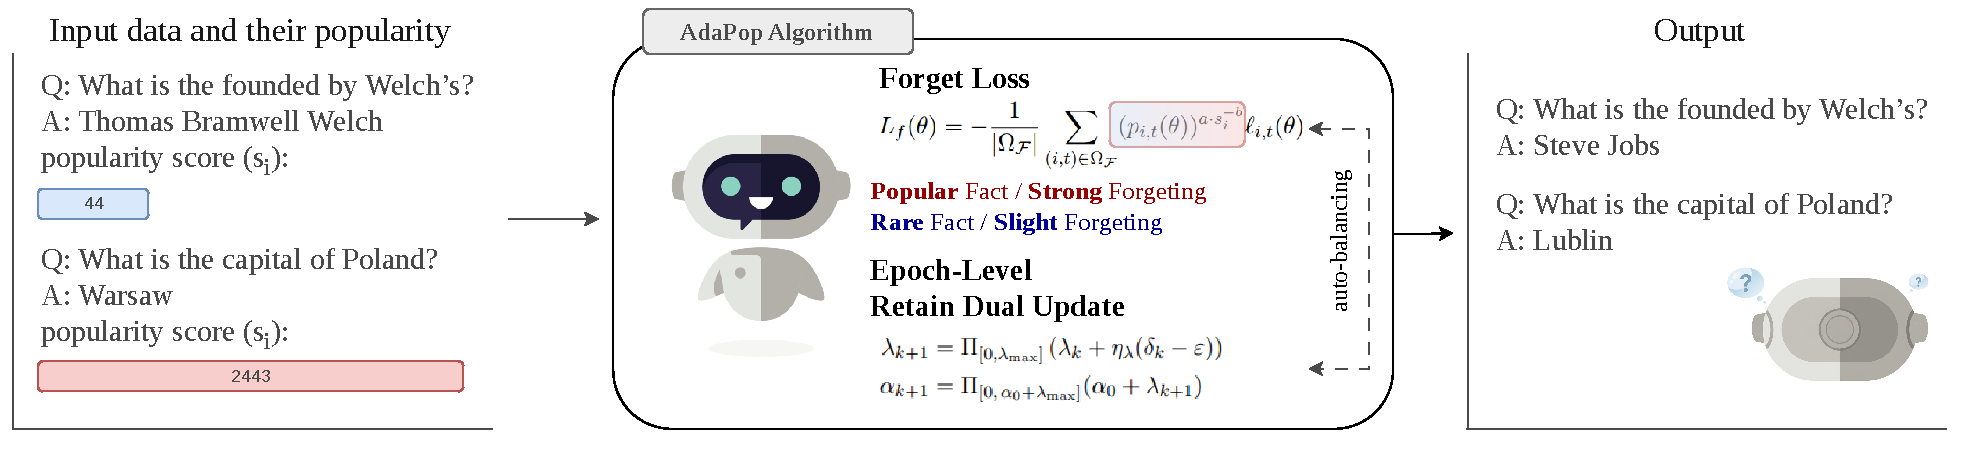
\includegraphics[width=0.85\textwidth]{latex/img/crop_adapop.pdf}
    %\caption{AdaPop assigns a per-fact exponent $\beta_i$ derived from an external popularity score, applying weaker unlearning to rare facts and stronger unlearning to popular ones. A dual-ascent controller adjusts the retain coefficient $\alpha$ at each epoch to keep retain-set loss within a preset tolerance.}
    \caption{Overview of AdaPop. The popularity exponent $\beta_i$ reweights per-fact token weights; the dual-ascent controller updates $\alpha$ each epoch to keep the retain loss within a preset tolerance $\varepsilon$.}
    \label{fig:adapop_workflow}
\end{figure*}

To address this issue, we introduce \textbf{AdaPop} (\textbf{Ada}ptive \textbf{Pop}ularity), a popularity-weighted adaptive gradient unlearning method (Figure~\ref{fig:adapop_workflow}) that conditions per-fact unlearning strength on an external popularity proxy and pairs this popularity scaling with an automated retain-balancing controller. AdaPop maps each forget example’s global popularity (e.g., inbound citelinks from Wikidata) to a per-fact exponent that reweights token ascent signals, then uses an epoch-level dual-ascent variable to enforce a bounded drift on a retain set. The novelty is two-fold: (1) explicit, externally-sourced popularity conditioning of per-fact gradient pressure, which directly addresses the popularity gap rather than proxying it via model confidence, and (2) an automated dual-ascent controller that operates on the popularity-weighted forget loss to find stable forget/retain operating points without dataset-specific tuning of loss weights. We empirically show AdaPop achieves deeper paraphrase-generalised erasure and larger internal representation disruption than competitive baselines while preserving general capabilities across multiple 7–8B LLM families and two real-world knowledge benchmarks, DUET~\cite{anna2026anatomy} and RWKU~\cite{jin2024rwku}.

\begin{comment}
To address this issue, we introduce \textbf{AdaPop} (\textbf{Ada}ptive \textbf{Pop}ularity), a popularity-weighted adaptive gradient unlearning method (Figure~\ref{fig:adapop_workflow}). AdaPop scales the gradient update for each forget-set fact according to its global popularity and automates the forget-retain balance via a dual-ascent controller. In a preprocessing stage, AdaPop uses Wikidata inbound citelink counts as a popularity annotator~\cite{anna2026anatomy} to assign each fact a per-fact exponent $\beta_i$ that controls the strength of its gradient update. Facts with a higher popularity score receive a stronger unlearning force; rare facts receive a weaker one.

We evaluate AdaPop against SOTA unlearning algorithms on two real-world knowledge benchmarks, DUET~\cite{anna2026anatomy} and RWKU~\cite{jin2024rwku}, across three model families (Llama-3.1-8B, Qwen2.5-7B, Gemma-7B). AdaPop consistently reduces forget-set ROUGE-L and cosine similarity below all baselines while keeping retain-set scores within the range of the unmodified model, with the largest gains on paraphrase-generalized and adversarial-robustness subsets, and with general language capabilities preserved throughout.

We further study the contribution of each AdaPop component through a controlled ablation (Appendix~\ref{app:ablation}), independently removing the popularity exponent $\beta_i$ and the dual-ascent controller. The results show that neither component alone accounts for the full gain: fixing $\alpha$ with dynamic $\beta_i$ is the worst-performing variant, while full AdaPop is the only configuration that produces both deep forget-set erasure and stable retain-set preservation across all models.

We hope AdaPop and our findings pave the way for future research on LLM unlearning via popularity salience.
\end{comment}

% \paragraph{Contributions.}
% \begin{itemize}
%     \item We confirm the \emph{popularity gap} as a systematic failure mode of confidence-based unlearning: methods calibrated on local model confidence under-erase popular facts while risking over-erasure of rare ones, a failure mode observed but not addressed by prior work~\cite{krishnannot, anna2026anatomy}.
%     \item We introduce \textbf{AdaPop}, which addresses this via (i) a popularity-dependent exponent $\beta_i$ derived from Wikidata to globally calibrate the unlearning signal per fact, and (ii) a dual-ascent controller that automatically adjusts the retain coefficient during training, eliminating manual hyperparameter search.
%     \item We evaluate AdaPop on DUET~\cite{anna2026anatomy} and RWKU~\cite{jin2024rwku} across three model families, showing that a global popularity signal produces deeper semantic erasure than local confidence-based methods across all models, with paraphrase-generalized forgetting as the clearest differentiator and general capabilities preserved throughout (§\ref{sec:main_results}--\ref{sec:lm_eval}).
% \end{itemize}

















% % VERSION 1
% Privacy regulations and the right to erasure create concrete demand for machine unlearning: removing specific knowledge from a trained model without retraining from scratch~\cite{mantelero2013eu, cao2015towards, bourtoule2021machine}. Large language models present a distinctive challenge. LLMs memorize substantial portions of their pretraining data~\cite{carlini2021extracting, tirumala2022memorization, carlini2023quantifying}, including personally identifiable information and sensitive facts, making post-hoc removal both practically necessary and technically difficult. The difficulty is not uniform: facts encountered frequently during pretraining are redundantly encoded across many layers and attention heads, making them far more resistant to gradient-based removal than rarely seen facts~\cite{kandpal2023large, hartmann2024undesirable, merullo2025linear}.

% Existing unlearning algorithms treat all facts in the forget set as equally hard to erase. Gradient Ascent (GA;~\citealt{jang2022knowledge}) maximizes the negative log-likelihood on the forget set without constraint, frequently causing catastrophic collapse of linguistic coherence~\cite{zhang2024negative}. Gradient Difference (GD;~\citealt{liu2022continual}) adds a retain loss but still assigns equal gradient weight to every forget token. Negative Preference Optimization (NPO;~\citealt{zhang2024negative}) reformulates unlearning as preference alignment, yielding a conservative signal that fails to erase well-memorized popular facts. Weighted Gradient Ascent (WGA;~\citealt{wang2025rethinking}) weights each token's gradient by the model's log-probability, concentrating unlearning on high-confidence tokens. All four methods calibrate the unlearning signal from the model's current output distribution, a quantity that changes throughout training and does not reflect how deeply a fact is parametrically encoded~\cite{hartmann2024undesirable, kandpal2023large}. The result is a systematic \emph{popularity gap}: methods calibrated for rare facts over-erase them while under-erasing popular ones, and vice versa.

% Krishnan et al.~\cite{krishnannot} confirm through controlled experiments across model scales that frequently encountered facts are either not unlearned at all or only superficially forgotten, remaining extractable via adversarial queries. Borisiuk et al.~\cite{anna2026anatomy} establish the same failure mode on the DUET benchmark, showing that fact salience systematically predicts unlearning difficulty across multiple gradient-based methods. Both works identify the problem empirically but offer no popularity-aware training method to address it.

% We introduce \textbf{AdaPop} (\textbf{Ada}ptive \textbf{Pop}ularity), which addresses this gap by conditioning gradient updates on an external popularity proxy and automating the forget-retain balance via a dual-ascent controller. As a popularity proxy, we use the sum of inbound Wikipedia citelinks to the subject and object nodes of each forget-set fact, computed from Wikidata (\texttt{pop\_sum}). This signal is static and independent of the model's current output distribution, providing stable per-fact calibration of unlearning strength. A dual-ascent controller adjusts the retain coefficient $\alpha$ at each training epoch to keep retain-set loss within a preset tolerance, eliminating manual hyperparameter search. Figure~\ref{fig:adapop_workflow} illustrates the full workflow.

% Through experiments on DUET~\cite{anna2026anatomy} and RWKU~\cite{jin2024rwku} across three model families (Llama-3.1-8B, Qwen2.5-7B, Gemma-7B), AdaPop produces deeper semantic erasure than all local confidence-based baselines, with the clearest gains on paraphrase-generalized forgetting metrics, while preserving general language capabilities across all settings.


% \begin{figure*}[t]
%     \centering
%     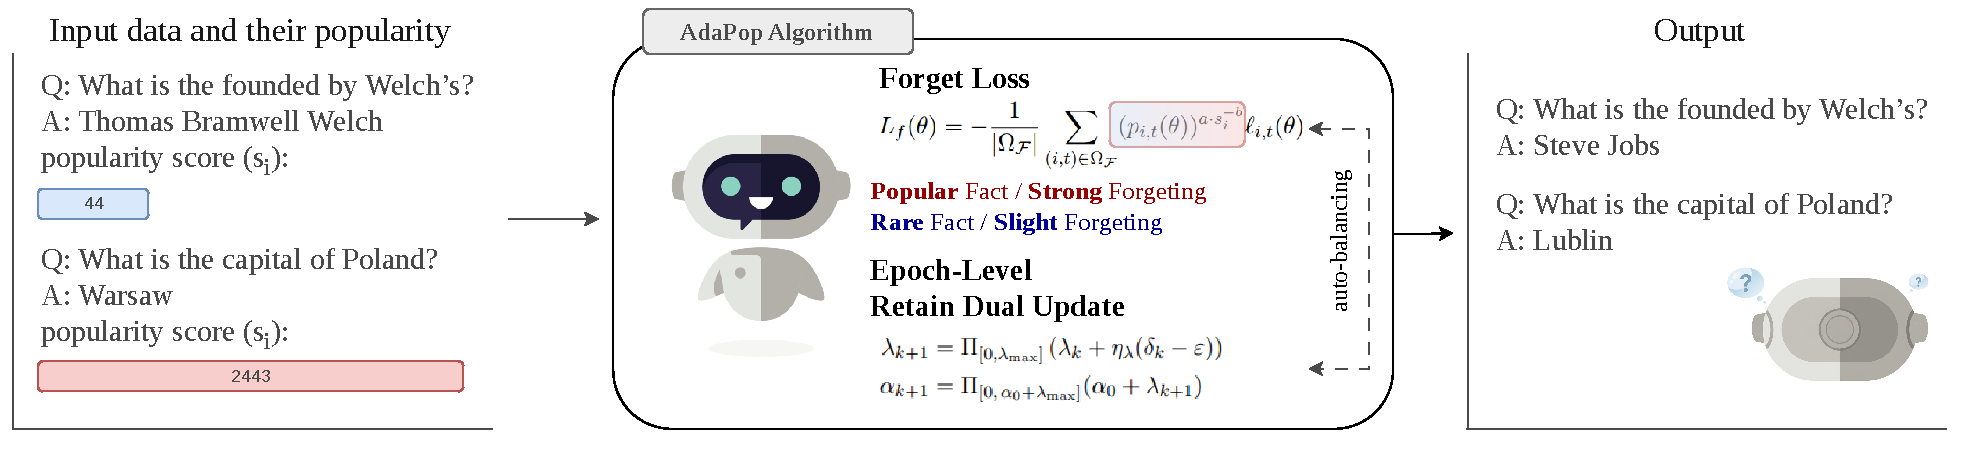
\includegraphics[width=0.85\textwidth]{latex/img/crop_adapop.pdf}
%     \caption{AdaPop assigns a per-fact exponent $\beta_i$ derived from an external popularity score, applying weaker unlearning to rare facts and stronger unlearning to popular ones. A dual-ascent controller adjusts the retain coefficient $\alpha$ at each epoch to keep retain-set loss within a preset tolerance.}
%     \label{fig:adapop_workflow}
% \end{figure*}


% \paragraph{Contributions.} We make the following contributions:
% \begin{itemize}
%     \item We confirm the \emph{popularity gap} as a systematic failure mode of confidence-based unlearning: methods calibrated on local model confidence under-erase popular facts while risking over-erasure of rare ones, a failure mode observed but not addressed by prior work~\cite{krishnannot, anna2026anatomy}.
%     \item We introduce \textbf{AdaPop}, which addresses this via (i) a popularity-dependent exponent $\beta_i$ derived from Wikidata to globally calibrate the unlearning signal per fact, and (ii) a dual-ascent controller that automatically adjusts the retain coefficient during training, eliminating manual hyperparameter search.
%     \item We evaluate AdaPop on DUET~\cite{anna2026anatomy} and RWKU~\cite{jin2024rwku} across three model families (Llama-3.1-8B, Qwen2.5-7B, Gemma-7B), showing that a global popularity signal produces deeper semantic erasure than local confidence-based methods across all models, with paraphrase-generalized forgetting as the clearest differentiator and general capabilities preserved throughout (§\ref{sec:main_results}--\ref{sec:lm_eval}).
% \end{itemize}









%% PLAN FROM 14/03/26
% %% Describe what is the problem current algos (stability isses, popularity influence): Gradient Ascent, Gradient Difference, NPO, WGA;
% %% Explain how we solve this popularity gap 
% %% Which benchmark we use to evaluate (we use real-world facts QA benchmarks for solving real-words tasks; we scoring facts based on they popularity. if you have ascess to pretrain set, you can use information from it to scoring populaeiry; otherwise use 'approximate' metrics from large data corpus like wikidata to score facts. here popularity is the global metric for for unlerning regularization; the local (model) metric is log probes and its to factors influence to unlearning.) also for trade-off stability we automatically balance retain, that directly effect to forgetting.

% %% добавить ссылки, можно посмотреть из интро статьи (https://arxiv.org/pdf/2504.05058)
% % Privacy regulations and the right to erasure create concrete demand for machine unlearning: the ability to remove specific facts from a trained model without retraining from scratch. In LLMs, however, removing a fact is not symmetric with inserting it.

% Cуществующие сота анлеарн методы ортимизируют лоссы типа преференс оптиизации \cite{NPO} и градиентной разницы \cite{GA, GD, WGA}.
% Эти methods rely on local model confidence as their primary signal, and none adjust the forget-retain balance dynamically. 
% Однако,не в токенам дело
% Таким образом, 
% проблемы методов на реал ворлд дата в том, что все точки одинаковые krishnannot и мы. Однако известно, что частота фактов влияет на меморизацию ссылка \cite{}.  

% To address the issue, мы предлагаем метод адаптивного анлергинга на популярности named adapop. As shown in Figure,. We introduce \textbf{AdaPop} (Adaptive Popularity), which addresses this gap by scaling gradient updates per fact using an external popularity proxy and automates the forget-retain balance via a dual-ascent controller. We introduce \textbf{AdaPop}, which addresses this via (i) a popularity-dependent exponent $\beta_i$ derived from Wikidata globally calibrate the unlearning signal per fact, and (ii) a dual-ascent controller that automatically adjusts the retain coefficient during training, eliminating manual hyperparameter search.


% Through extensive experiments across two benchmarks such as DUET and RWKU, we demonstrate constant improvement on forget set while preserving retain results. В частности, цифраю 

% %Facts encountered frequently during pretraining are redundantly encoded across many layers and attention heads, making them far more resistant to gradient-based removal than rarely encountered facts. Existing algorithms treat all facts in the forget set as equally hard to erase, producing a systematic popularity gap: methods calibrated for rare facts over-erase them while under-erasing popular ones, and methods calibrated for popular facts risk collateral damage to rare knowledge and general capabilities \cite{anna2026anatomy, krishnannot}.

% %Gradient Ascent (GA, \cite{jang2022knowledge}) maximizes loss on the forget set without constraint, which frequently leads to catastrophic collapse of linguistic coherence. Gradient Difference (GD, \cite{liu2022continual}) adds a retain loss but still treats every forget token as equally important. Negative Preference Optimization (NPO, \cite{zhang2024negative}) reformulates unlearning as preference alignment, yielding a conservative signal that fails to erase well-memorised popular facts. Weighted Gradient Ascent (WGA, \cite{wang2025rethinking}) weights gradient updates by the model's own log-probabilities, focusing ascent on high-confidence tokens. All above-mentioned methods rely on local model confidence as their primary signal, and none adjust the forget-retain balance dynamically. The result is a suboptimal tradeoff: methods must be hand-tuned per dataset and model to avoid either insufficient forgetting or retain-set degradation. Our central claim is that log-probabilities alone do not accurately reflect how deeply a fact is embedded in the model~\cite{hartmann2024undesirable, kandpal2023large}; an external global popularity proxy provides a more reliable signal for calibrating unlearning strength.

% \begin{figure}[ht!]
%     \centering
%     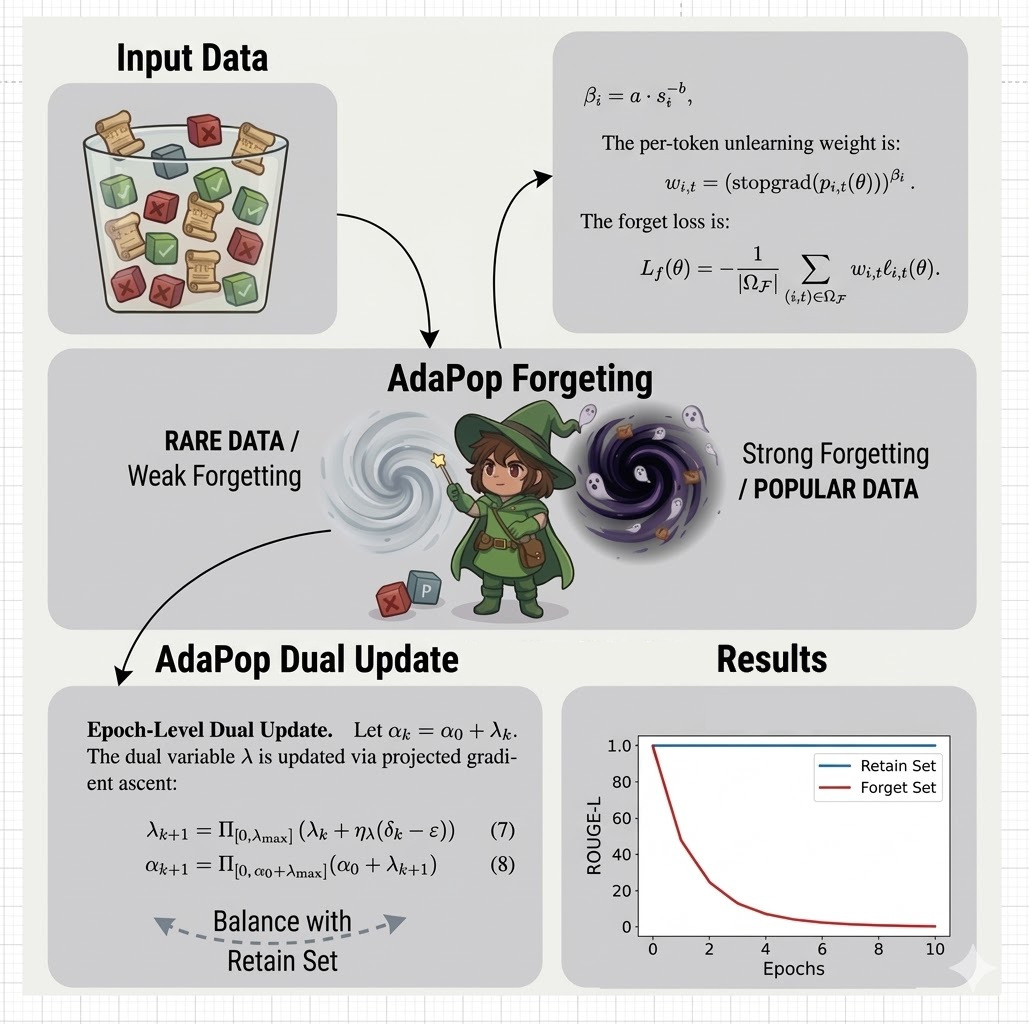
\includegraphics[width=1\linewidth]{latex/img/ada_pop_sq_illustr.jpg}
%     \caption{The proposed AdaPop assigns a per-fact exponent $\beta_i$ from an external popularity score, applying weaker unlearning to rare facts and stronger unlearning to popular ones. A dual-ascent controller adjusts the retain coefficient $\alpha$ at each epoch to keep retain-set loss within a preset tolerance.}
%     \label{fig:adapop_workflow}
% \end{figure}


%  As a popularity proxy, we use the sum of inbound citelinks (Wikipedia page references) to an entity's subject and object nodes, computed directly from Wikidata for each fact in the forget set; this quantity is Wikidata \texttt{pop\_sum}.

% \paragraph{Our contributions:} %We make the following contributions:
% % (Figure~\ref{fig:adapop_workflow})
% \begin{itemize}
%     \item We confirm the \emph{popularity gap} as a systematic failure mode of confidence-based unlearning: methods that calibrate updates on local model confidence under-erase popular facts (high memory inertia) while risking over-erasure of rare ones.

%     \item  We design a method for factuality-aware MU that trains something на частоте.    %\item We introduce \textbf{AdaPop}, which addresses this via (i) a popularity-dependent exponent $\beta_i$ derived from external knowledge bases (e.g., Wikidata) to globally calibrate the unlearning signal per fact, and (ii) a dual-ascent controller that automatically adjusts the retain coefficient during training, eliminating manual hyperparameter search.
    
%     %\item We evaluate \textbf{AdaPop} on DUET~\cite{anna2026anatomy} and RWKU~\cite{jin2024rwku} datasets across three models from different families (Llama-3.1-8B, Qwen2.5-7B, Gemma-7B), showing that a global popularity signal produces deeper semantic erasure than local confidence-based methods across all models, with paraphrase-generalised forgetting as the clearest differentiator and general capability preserved throughout (§\ref{sec:main_results}--\ref{sec:lm_eval}).
%     \item We demonstrate that on two benchmark datasets, our method outperforms state-of-the-art on both MU and erase/attack metrics.

% \end{itemize}

